\documentclass[
	classe=$2^{de}$,
	headerTitle=Généralités\space sur\space les\space vecteurs
]{coursclass}

\usetikzlibrary{calc}

\title{Chapitre 3 : Généralités sur les vecteurs}
\date{}
\author{}

\begin{document}

\maketitle

\begin{definition}[Vecteurs]
	Toute translation du plan est associée à un \textbf{vecteur}, qui représente le déplacement des points occasionné par la translation. Un vecteur est entièrement déterminé par :
	\begin{itemize}
		\item Sa \textbf{direction}.
		\item Son \textbf{sens}.
		\item Sa longueur, qu'on appelle sa \textbf{norme}.
	\end{itemize}
\end{definition}

\begin{exemple}
	\begin{multicols}{2}
		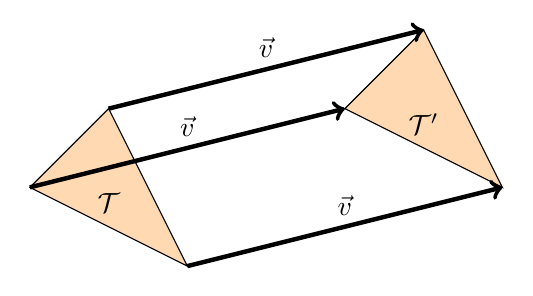
\begin{tikzpicture}
			\coordinate (A) at (0,0);
			\coordinate (B) at ($(A)+(2,-1)$);
			\coordinate (C) at ($(A)+(1,1)$);
			\coordinate (A') at (4,1);
			\coordinate (B') at ($(A')+(2,-1)$);
			\coordinate (C') at ($(A')+(1,1)$);

			\draw[fill=orange!30] (A) -- (B) -- (C) -- cycle;
			\node at ($(A)+(1,-0.2)$) {$\mathcal{T}$};
			\draw[fill=orange!30] (A') -- (B') -- (C') -- cycle;
			\node at ($(A')+(1,-0.2)$) {$\mathcal{T}'$};

			\draw[ultra thick,->] (A) -- node[midway,above] {$\vec{v}$} (A');
			\draw[ultra thick,->] (B) -- node[midway,above] {$\vec{v}$} (B');
			\draw[ultra thick,->] (C) -- node[midway,above] {$\vec{v}$} (C');

		\end{tikzpicture}

		\columnbreak

		Sur la figure ci-contre, le triangle $\mathcal{T}'$ est l'image du triangle $\mathcal{T}$ par la translation de vecteur $\vec{v}$.
	\end{multicols}
\end{exemple}

\begin{definition}[Égalité de vecteurs]
	Deux vecteurs sont \textbf{égaux} si ils ont la même direction, le même sens et la même norme.

	Dans ce cas, ils correspondent à la même translation.
\end{definition}

\begin{exemple}
	\begin{multicols}{2}
		\begin{tikzpicture}
			\draw[->] (0,0) -- node[midway,above] {$\vec{v}₁$} ++(3,1);
			\draw[->] (1,-1) -- node[midway,above] {$\vec{v}₂$} ++(3,1);
		\end{tikzpicture}

		\columnbreak

		Les vecteurs $\vec{v}₁$ et $\vec{v}₂$ sont \textit{égaux}.
	\end{multicols}
	\hrule

	\begin{multicols}{2}
		\begin{tikzpicture}
			\draw[->] (0,0) -- node[midway,above left] {$\vec{v}₁$} ++(2,2);
			\draw[->] (1,0) -- node[midway,above] {$\vec{v}₂$} ++(3,1);
		\end{tikzpicture}

		\columnbreak

		Les vecteurs $\vec{v}₁$ et $\vec{v}₂$ sont \textit{différents} : leur \uline{direction} n'est pas la même.
	\end{multicols}
	\hrule

	\begin{multicols}{2}
		\begin{tikzpicture}
			\draw[->] (0,0) -- node[midway,above] {$\vec{v}₁$} ++(3,1);
			\draw[->] (4,0) -- node[midway,above] {$\vec{v}₂$} ++(-3,-1);
		\end{tikzpicture}

		\columnbreak

		Les vecteurs $\vec{v}₁$ et $\vec{v}₂$ sont \textit{différents} : leur \uline{sens} n'est pas le même.
	\end{multicols}
	\hrule

	\begin{multicols}{2}
		\begin{tikzpicture}
			\draw[->] (0,0) -- node[midway,above] {$\vec{v}₁$} ++(3,1);
			\draw[->] (1,-1) -- node[midway,above] {$\vec{v}₂$} ++(2,2/3);
		\end{tikzpicture}

		\columnbreak

		Les vecteurs $\vec{v}₁$ et $\vec{v}₂$ sont \textit{différents} : leur \uline{norme} n'est pas la même.
	\end{multicols}
\end{exemple}

\begin{definition}[Vecteurs opposés]
	Si deux vecteurs ont la même direction, la même norme, mais des sens différents, on dit qu'ils sont \textbf{opposés}.
\end{definition}

\begin{vocabulaire}
	\begin{center}
		\begin{tikzpicture}
			\coordinate (A) at (0,0);
			\coordinate (B) at (3,1.5);

			\node[above] at (A) {A};
			\node[above] at (B) {B};
			\draw[->] (A) -- node[midway,above left] {$\widevec{AB}$} (B);
		\end{tikzpicture}
	\end{center}

	Si une translation envoie le point A sur le point B, on peut appeller le vecteur de cette translation \squareFrame{$\widevec{AB}$}.
\end{vocabulaire}

\begin{definition}[Somme de vecteurs]
	Soient deux vecteurs $\vec{u}$ et $\vec{v}$. Si on enchaîne les translations correspondant à $\vec{u}$ et à $\vec{v}$, on obtient une nouvelle translation.

	Le vecteur qui lui est associé est appelé la \textbf{somme de $\vec{u}$ et de $\vec{v}$}. On la note \squareFrame{$\vec{u} + \vec{v}$}.
\end{definition}

\begin{exemple}
	\begin{center}
		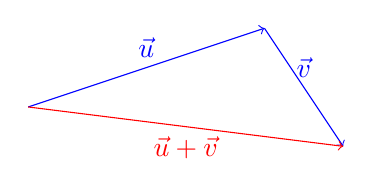
\begin{tikzpicture}
			\coordinate (A) at (0,0);
			\coordinate (B) at (3,1);
			\coordinate (C) at (4,-0.5);

			\draw[blue,->] (A) -- node[above] {$\vec{u}$} (B);
			\draw[blue,->] (B) -- node[above] {$\vec{v}$} (C);
			\draw[red,->] (A) -- node[below] {$\vec{u}+ \vec{v}$} (C);
		\end{tikzpicture}
	\end{center}
\end{exemple}

\begin{remarque}
	L'ordre de la somme n'importe pas : $\vec{u} + \vec{v} = \vec{v} + \vec{u}$.
\end{remarque}

\begin{propriete}[Relation de Chasles]
	Soient $A$, $B$ et $C$ trois points. On a
	$$ \widevec{A{\color{red}B}} + \widevec{{\color{red}B}C} = \widevec{AC} $$
\end{propriete}

\end{document}